\section{Nanosheets}

\paragraph{Creation process: }

The standard model is created in Blender using a cube with a central subdivision along the Y axis. It is centred in the origin with half size equal to 1. The geometrical shape of a nanosheet is well defined \cite{angleTIO2} with an angle of 68.3° obtained from anatase $TiO_2$ X-ray measurements. This recurring feature gives us the possibility to generate a standard, unitary-sized, model to use as a template for all the future instances.
The final model is obtained after a series of steps applied to the template model, as shown in Fig. \ref{fig:nano_creation}:
%
\begin{itemize}
    \item Scale along Y axis (to match the correct ratio between height and width) equals to: $S_Y = h / w$
    \item Scale along XZ plane (to generate the insets of the superior and inferior faces) equals to: $S_{XZ} = 1 - (h_{\text{eff}} / tan(68.3^{\circ}))$
\end{itemize}
%
Where h\_eff is the new calculated height.

\begin{figure}[ht]
    \centering
    \begin{subfigure}[b]{0.32\textwidth}
        % nano_1_1
        \includegraphics[width=.95\textwidth]{./immagini/nano_1_1.png}
        \caption{}
        \label{fig:nano_creation_a}
    \end{subfigure}
    \hfill
    \begin{subfigure}[b]{0.32\textwidth}
        % nano_1_2
        \includegraphics[width=.95\textwidth]{./immagini/nano_1_2.png}
        \caption{}
        \label{fig:nano_creation_b}
    \end{subfigure}
    \hfill
    \begin{subfigure}[b]{0.32\textwidth}
        % nano_1_3
        \includegraphics[width=.95\textwidth]{./immagini/nano_1_3.png}
        \caption{}
        \label{fig:nano_creation_c}
    \end{subfigure}
    \caption{Creation of steps: a) Scale along Y axis, b) Inset of the superior and inferior surfaces c) Final standard model}
    \label{fig:nano_creation}
\end{figure}

\paragraph{Positioning process: }

The additional information provided enables us to execute additional steps. This will include passages such as: floor process, positioning, rotation and scale, as shown in Fig. \ref{fig:nano_pos}:


\begin{itemize}
    \item The standard model is centered in the world origin, this means that we need to floor it (position the model so it will not clip with the floor substrate).
    \item Given the different size of the particle can be scaled accordingly, remembering that the half size of the standard model is equal to 1. This means we need to scale everything by a factor of (nominal\_size / 2).
    \item Now that the particle is generated and resized it now possible to traslate it by a vector $\vec{v}$ = (x, z) on the floor.
\end{itemize}

\begin{figure}[ht]
    \centering
    \begin{subfigure}[b]{0.32\textwidth}
        % nano_2_1
        \includegraphics[width=.95\textwidth]{./immagini/nano_2_1.png}
        \caption{}
        \label{fig:nano_pos_a}
    \end{subfigure}
    \hfill
    \begin{subfigure}[b]{0.32\textwidth}
        % nano_2_2
        \includegraphics[width=.95\textwidth]{./immagini/nano_2_2.png}
        \caption{}
        \label{fig:nano_pos_b}
    \end{subfigure}
    \hfill
    \begin{subfigure}[b]{0.32\textwidth}
        % nano_2_3
        \includegraphics[width=.95\textwidth]{./immagini/nano_2_3.png}
        \caption{}
        \label{fig:nano_pos_c}
    \end{subfigure}
    \caption{Creation of steps: a) Scale along Y axis, b) Inset of the superior and inferior surfaces c) Final standard model}
    \label{fig:nano_pos}
\end{figure}

\newpage

\paragraph{Examples: }

Some examples of generated images are reported in Fig. \ref{fig:nanosheet}a-c. In particular, Fig. \ref{fig:nanosheet_b} and \ref{fig:nanosheet_c} show compenetrated nanosheets, that are successfully handled by this system.

\begin{figure}[ht]
    \centering
    \begin{subfigure}[b]{0.32\textwidth}
        % nanosheet_singola
        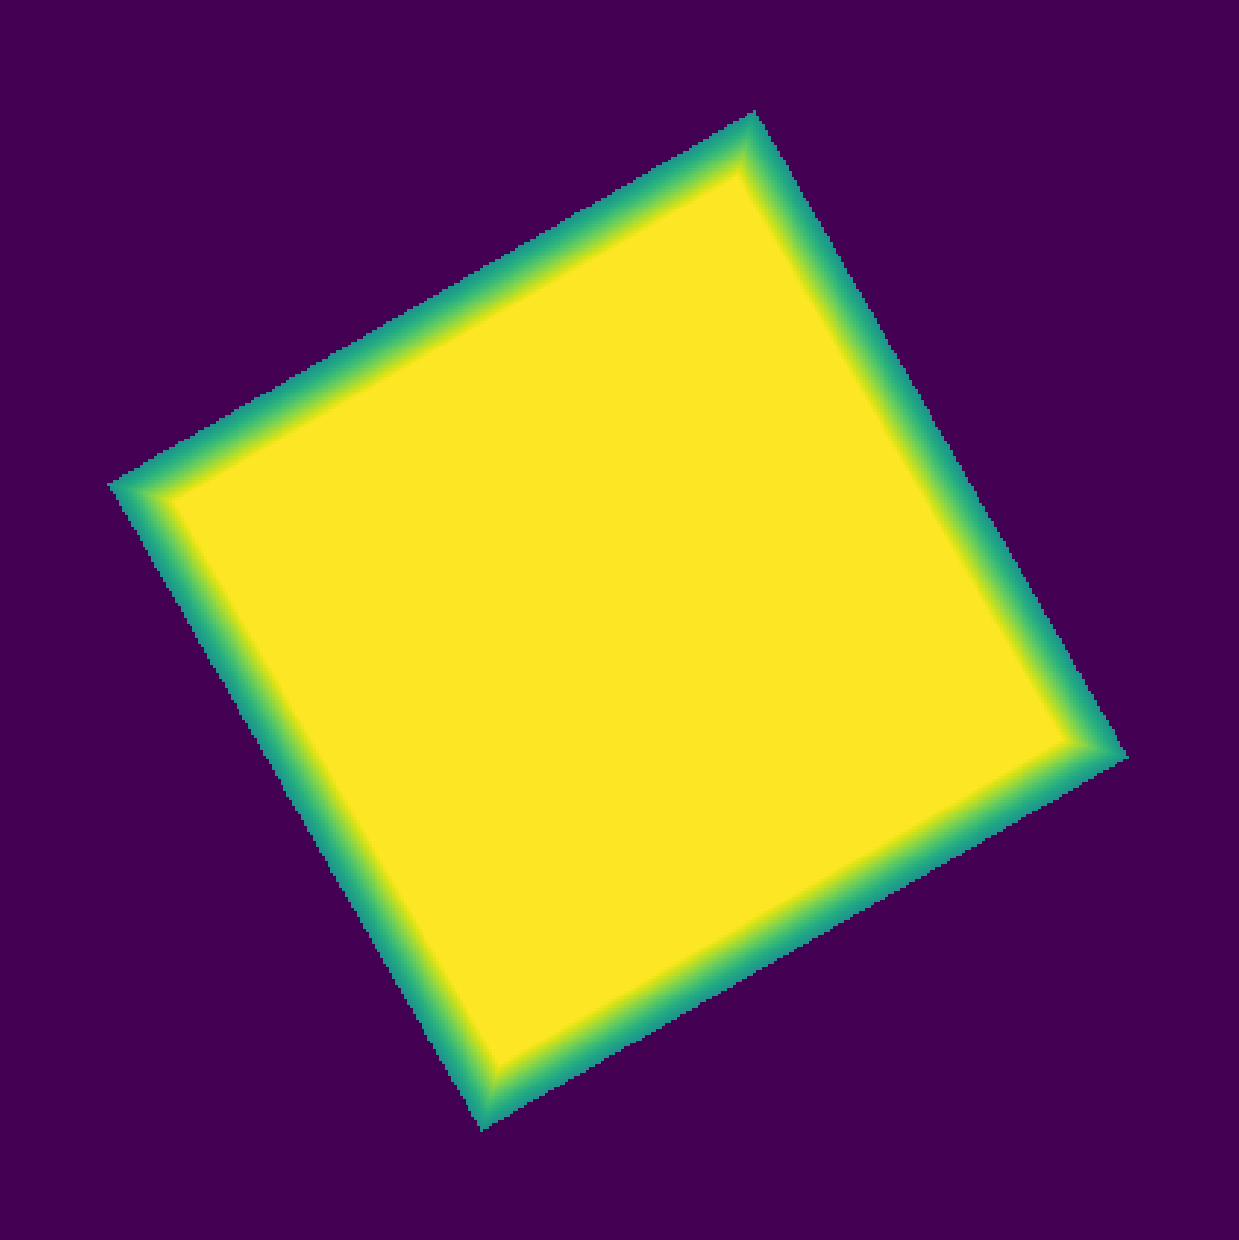
\includegraphics[width=.95\textwidth]{./immagini/nanosheet_singola.png}
        \caption{}
        \label{fig:nanosheet_a}
    \end{subfigure}
    \hfill
    \begin{subfigure}[b]{0.32\textwidth}
        % nanosheet_doppia
        
\includegraphics[width=.95\textwidth]{./immagini/nanosheet_doppia.png}
        \caption{}
        \label{fig:nanosheet_b}
    \end{subfigure}
    \hfill
    \begin{subfigure}[b]{0.32\textwidth}
        % nanosheet_statistica
        
\includegraphics[width=.95\textwidth]{./immagini/nanosheet_statistica.png}
        \caption{}
        \label{fig:nanosheet_c}
    \end{subfigure}
    \caption{a) Single, b) Double and  c) Statistic used nanosheets}
    \label{fig:nanosheet}
\end{figure}